\chapter{Vergleich der verschiedenen Implementierungen}
\label{chapter:4}

Nun wollen wir die implementierten Algorithmen im Bezug auf ihre Laufzeit miteinander vergleichen. Die Berechnung der Laufzeiten erfolgt erneut mit einem Python-Skript. Dieses Skript führt die jeweilige Regression über einen Kommandozeilenbefehl aus und misst die Zeit dieser Operation. Die Anzahl der Wiederholungen und die Anzahl der verwendeten Datenpunkte können als Parameter übergeben werden. Das Skript findet man im Anhang unter \ref{appendix:F:1}.

Die Laufzeiten der Berechnungen werden als csv-Datei gespeichert. Pro Berechnung wird eine Zeile in die Ergebnisdatei geschrieben. Diese Zeile enthält die Programmiersprache, die Art der Regression, die Anzahl der verwendeten Datenpunkte und die Dauer der Berechnung.

Für jede Kombination der ersten drei Werte wurden 100 Berechnungen durchgeführt, falls die Dauer einer Berechnung höchstens 100 Sekunden betrug. Für Berechnungen, die länger als 100 Sekunden dauerten, wurde die Anzahl auf 50 Berechnungen reduziert. Skripte mit einer Laufzeit von länger als 1000 Sekunden wurden nur zehn mal ausgeführt. Für das Benchmarking wurde ein MacBook Pro (Mitte 2012, Betriebssystem macOS High Sierra 10.13.2) mit einem 2,9 GHz Intel Core i7 Prozessor und 8 GB 1600 MHz DDR3 Arbeitsspeicher verwendet.

Auch für das Auswerten der berechneten Benchmarks wurde ein Python-Skript erstellt, welches im Anhang \ref{appendix:F:2} abgedruckt ist. Dieses Skript liest die csv-Datei mit Benchmarks ein und gibt eine Tabelle mit den durchschnittlichen Laufzeiten pro Art der Regression, Programmiersprache und Anzahl verwendeter Datenpunkte aus. Außerdem wird pro Typ der Regression ein Plot zum Vergleich der Laufzeiten erzeugt.

\section{Einfache lineare Regression}
\label{section:4:1}

Folgende Ergebnisse erhalten wir bei einfacher linearer Regression:

\begin{center}
  \captionof{table}{Laufzeiten in Sekunden für einfache lineare Regression}
  \begin{tabular}{|c|c|c|c|c|c|}\hline
    & \textbf{10} & \textbf{100} & \textbf{1000} & \textbf{10000} & \textbf{100000} \\ \hline
    \textbf{r} & 0.38453477 & 0.40336191 & 0.38638819 & 0.40475887 & 0.54730985 \\ \hline
    \textbf{tensorflow} & 2.96190362 & 2.94665535 & 3.00290149 & 3.69807061 & 7.73616447 \\ \hline
    \textbf{mysql} & 0.02591379 & 0.02506811 & 0.03348756 & 0.11362195 & 0.82149320 \\ \hline
    \textbf{postgresql} & 0.03092405 & 0.03056195 & 0.03340294 & 0.04948901 & 0.21394655 \\ \hline
  \end{tabular}
\end{center}

Der zugehörige Graph sieht folgendermaßen aus:

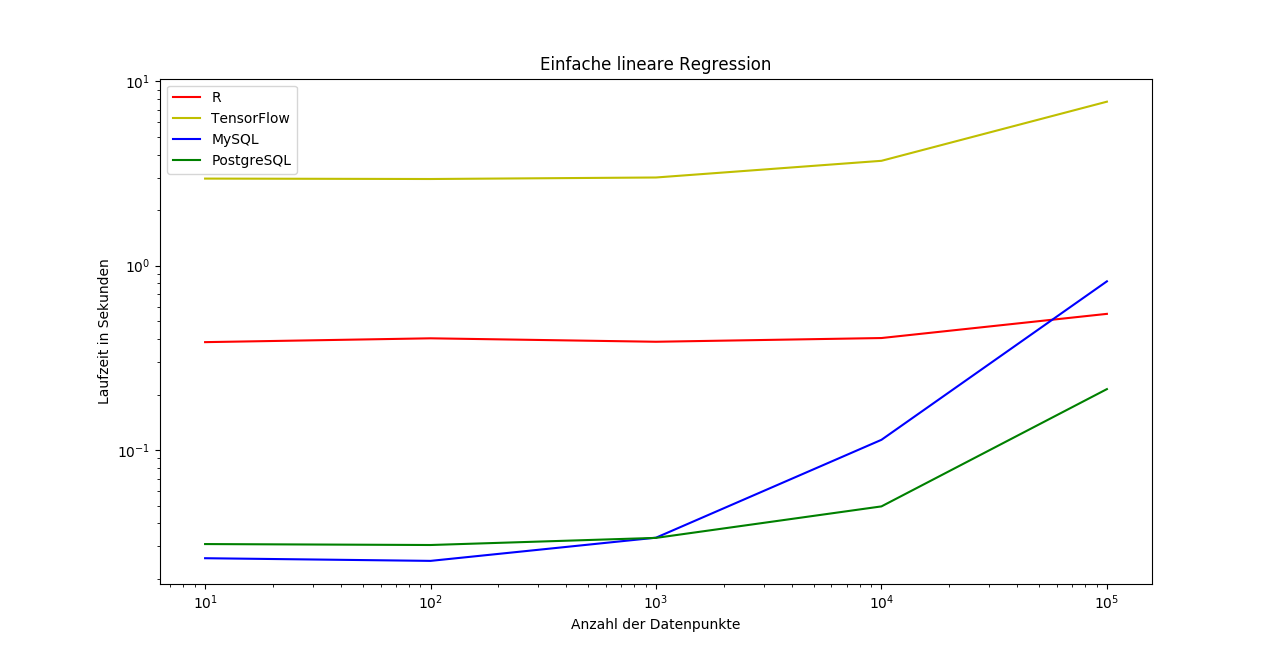
\includegraphics[width=\textwidth]{simpleLinearRegressionBenchmark}

TensorFlow und R haben eine relativ konstante Lautzeit, auch bei größeren Datenmengen. Dabei ist TensorFlow mit iterativer Berechnung wie erwartet mit Abstand am langsamsten. Die SQL-Implementierungen sind bei geringer Anzahl an Datenpunkten sogar die schnellsten Skripte. Für größer werdende Datenmengen erkennt man aber einen rapiden Anstieg in der Laufzeit.

\section{Multiple lineare Regression}
\label{section:4:2}

Die Skripte für multiple lineare Regression besitzen folgende Laufzeiten:

\begin{center}
  \captionof{table}{Laufzeiten in Sekunden für multiple lineare Regression}
  \begin{tabular}{|c|c|c|c|c|c|}\hline
    & \textbf{10} & \textbf{100} & \textbf{1000} & \textbf{10000} & \textbf{100000} \\ \hline
    \textbf{r} & 0.38108478 & 0.37967851 & 0.38452695 & 0.39888490 & 0.54517789 \\ \hline
    \textbf{tensorflow} & 167.220486 & 168.885465 & 168.668689 & 168.821214 & 169.254182 \\ \hline
    \textbf{mysql} & 0.04174929 & 0.05248516 & 0.15990342 & 1.09634777 & 10.8214030 \\ \hline
    \textbf{postgresql} & 0.03053954 & 0.03336087 & 0.05904620 & 0.30572490 & 2.71992954 \\ \hline
  \end{tabular}
\end{center}

Das geplottete Ergebnis sieht wie folgt aus:

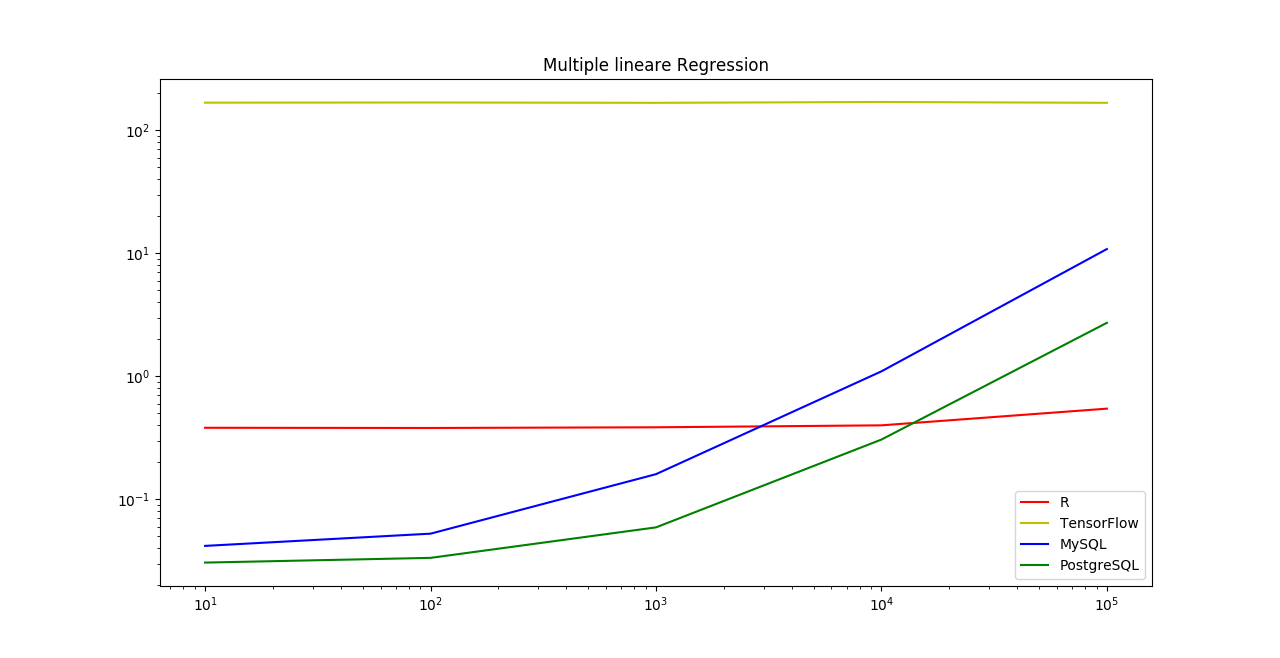
\includegraphics[width=\textwidth]{multipleLinearRegressionBenchmark}

Hier zeigt sich ein ähnliches Bild wie schon bei einfacher linearer Regression. Wieder liefern R und TensorFlow relativ konstante Laufzeiten, wobei die Laufzeit des TensorFlow-Skriptes wegen der $50000$ durchgeführten Iterationen dieses Mal extrem langsam ist. Wieder sind die SQL-Skripte bei kleinen Datenmengen am schnellsten. Bei größeren Datenmengen werden sie allerdings von R geschlagen. Interessant ist außerdem, dass die PostgreSQL-Implementierung noch schneller als die Variante in MySQL. Die Arrays in PostgreSQL arbeiten also effizienter als die temporären Relationen in MySQL.

\section{Logistische Regression}
\label{section:4:3}

Betrachten wir zuletzt noch die Laufzeiten für logistische Regression:

\begin{center}
  \captionof{table}{Laufzeiten in Sekunden für logistische Regression}
  \begin{tabular}{|c|c|c|c|c|c|}\hline
    & \textbf{10} & \textbf{100} & \textbf{1000} & \textbf{10000} & \textbf{100000} \\ \hline
    \textbf{r} & 0.40403676 & 0.39953323 & 0.40047518 & 0.43356463 & 0.91014730 \\ \hline
    \textbf{tensorflow} & 2.88191271 & 2.88278436 & 2.92470042 & 3.37794654 & 6.87024382 \\ \hline
    \textbf{mysql} & 1.57908838 & 4.51631200 & 35.3472805 & 283.849979 & 2680.43056 \\ \hline
    \textbf{postgresql} & 3.73521209 & 48.8452754 & 521.625671 & 5175.87997 &  \\ \hline
  \end{tabular}
\end{center}

Die Visualisierung der Tabelle sieht so aus:

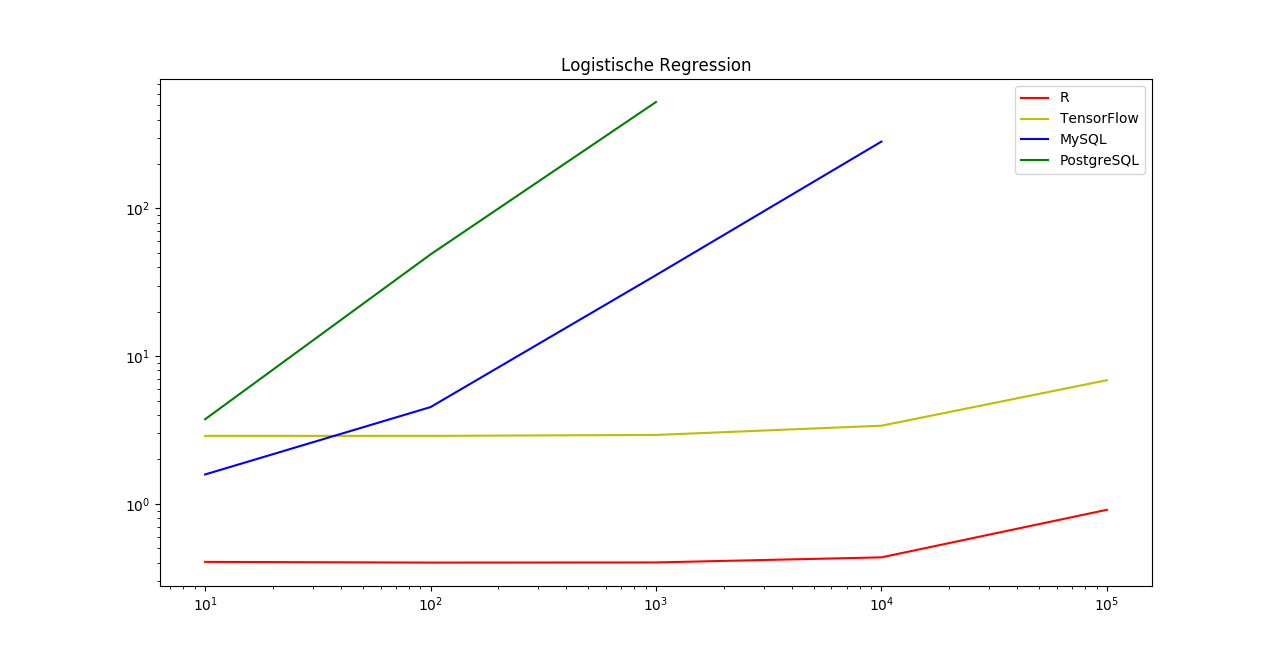
\includegraphics[width=\textwidth]{logisticRegressionBenchmark}

Wieder erkennt man eine Ähnlichkeit zu den vorherigen Diagrammen. Die SQL-Implementierungen sind nun aber von Anfang an deutlich langsamer als die Skripte in R und TensorFlow. Die Laufzeit steigt außerdem sehr schnell weiter an. So wurden für $100000$ Datenpunkte in PostgreSQL gar keine Benchmarks mehr berechnet, da die erwartete Laufzeit etwa $50000$ Sekunden, also knapp $14$ Stunden beträgt. Klarer Gewinner ist hier R, wo auch $100000$ Datenpunkte in weniger als einer Sekunde verarbeitet werden können.
